% \renewcommand{\sepCapaTitulo}{Gerenciar OS ASSEL}
% \renewcommand{\sepCapaData}{18 de Julho de 2022}
% \renewcommand{\sepCapaFile}{sep-capa-verde.pdf}

\chapter{Gerenciar OS Assel}
\label{detalhes:ger-os-assel}


A funcionalidade ``Gerenciar OS pela ASSEL'' é composta de 3 janelas: uma janela principal e duas janelas auxiliares. 

A janela principal já foi apresentada em reuniões. Esse documento pretende detalhar as duas demais janelas: A Janela Detalhes e a Janela Analisar. A primeira deve apresentar o histórico de uma Solicitação enquanto a outra auxilia os servidores da ASSEL no processo de análise das solicitações e tomada de providências decorrentes.

\section*{Alterações}


\begin{center}
	\begin{tabular}{|c|p{0.4\textwidth}|c|}
		\hline
		\rowcolor{lightgray!50} \multicolumn{3}{|c|}{\Large Alterações \normalsize} \\ \hline \hline
		% CABEÇALHO        
		\rowcolor{lightgray}\textbf{Data e Hora} & \textbf{Alterações} & \textbf{Hash do Commit}  \\ \hline
		% CONTEÚDO
		% Código escrito manualmente
		\rowcolor{corCOULD!10} 18/07/2022 11:30:00 & Alterei atributos do Artefato Andamento, Criação Artefato Observações & 11380ad \\ \hline			
	\end{tabular}    
\end{center}




\section{Janela Detalhes}

	A janela abre ao clicar em ``Detalhar''. A idéia é abrir os Detalhes de uma determinada Solicitação em uma nova aba do navegador de forma que o usuário possa abrir os detalhes de quantas solicitações quiser ao mesmo tempo. Assim, será fácil compará-las, analisar seu histórico e acessar seus arquivos.

	Deste modo, a janela de detalhes deve trazer todas as informações relacionadas à Solicitação desde sua criação até chegar onde chegou.
	
	Palavras Chave: Cronologia, Protocolo.

	\begin{funcionalidade}{Atenção: Essa ``janela'' deve abrir em nova aba do navegador}
		Essa janela deve ser aberta em nova aba pois quero que seja possível abrir abas distintas com solicitações distintas e comparar umas com as outras.
	\end{funcionalidade}		

	\subsection{1 - Cabeçalho - Informações Fixas sobre a OS}
		Informações fixas da Solicitação que deve aparecer no cabeçalho da janela.


		\begin{env-cor}{Informações da Solicitação}{cldfD}
			\begin{itemize}
				\item Solicitação
				\item Unidade Solicitante
				\item Tipo
				\item Subtipo
				\item Número da Proposição se MPAR
				\item Ano da Proposição se MPAR
				\item Comissão se MPAR
				\item Urgente
			\end{itemize}
		\end{env-cor}

		Dispor essas informações na tela parecido com a função Visualizar do Solicitar OS.
		
		
	\subsection{2 - Histórico ou Protocolo ou Cronologia}

	Em baixo do cabeçalho, deve ser possível ver \textbf{cronologicamente} as unidades por onde a solicitação passou, andamentos, ações realizadas, arquivos adicionados.
	
	Isto seria possível com um \emph{treeview} com 3 níveis conforme exemplo abaixo:

	
    \begin{figure}[htbp!]
	\dirtree{%
		.1 Solicitação MP001PLC-2021.
		.2 \msUnd Gab10 \DTcomment{01/08/21 14:16:25}. 
			.3 \msArt Arquivo1.png.
			.3 \msArt Arquivo2.png.
			.3 \msAnd Nova Solicitação.
		.2 \msUnd ASSEL \DTcomment{05/08/21 15:20:45}.
			.3 \msArt Arquivo3.pdf.
			.3 \msArt Arquivo4.pdf.
			.3 \msAct Vinculado à OS PELO010J1-2020. 
			.3 \msAct Desvinculado à PELO010J1-2020. 
			.3 \msAct Subtipo Modificado. 
			.3 \msAct Vinculado à OS PLC010J1-2020. 
			.3 \msAnd Solicitação de Pendência.
		.2 \msUnd Gabinete 10 \DTcomment{09/08/21 10:21:12}.
			.3 \msArt Pendencia.pdf.
			.3 \msAnd Resolução de Pendência.
		.2 \msUnd ASSEL \DTcomment{10/08/21 12:20:45}.
			.3 \msAnd Distribuição para UDA.
		.2 \msUnd UDA \DTcomment{10/08/21 18:20:45}.
			.3 \msAnd Solicitação de Redistribuição.
		.2 \msUnd ASSEL \DTcomment{11/08/21 10:00:10}.
			.3 \msAnd Distribuição para UCJ.
	}	
	\caption{Exemplo de Vista em Árvore}
	\label{tree:ex1}
	\end{figure}

	\newpage

    \begin{figure}[htbp!]
	\dirtree{%
		.2 \msUnd UCJ \DTcomment{12/08/21 08:30:00}.
			.3 \msAct Atribuído para Consultor Legislativo Titular.
			.3 \msAct Consultor Legislativo Titular Iniciou Elaboração.
			.3 \msArt Resultado.doc.
			.3 \msAct Atribuído para Consultor Legislativo Revisor.
			.3 \msAct Consultor Legislativo Revisor Iniciou Revisão.
			.3 \msArt Revisao.doc.
			.3 \msAct Atribuído para Consultor Legislativo Titular.
			.3 \msAct Consultor Legislativo Titular Finalizou Elaboração.
			.3 \msArt Final.doc.
			.3 \msAct Atribuído para Chefe Aprovar.
			.3 \msAct Chefe de Unidade Aprovou. 
			.3 \msAnd Notificação de Conclusão. 
		.2 \msUnd ASSEL \DTcomment{20/09/21 16:40:00}.
			.3 \msAct Artefatos Aprovados.
			.3 \msAnd Entrega para Solicitante.
		.2 \msUnd GAB10 \DTcomment{24/09/21 10:00:00}.
			.3 \msAct Download dos Artefatos.	
	}
	\caption{Continuação...}
	\label{tree:ex2}
	\end{figure}	
	
	
	As figuras \ref{tree:ex1} e \ref{tree:ex2} ilustram um exemplo de como seria o \emph{TreeView} de uma solicitação hipotética.
	
	Neste exemplo hipotético, ao observar a árvore podemos descrever o início da sequência cronológica de eventos dessa Solicitação:
	
	\begin{enumerate}
		\item Dia 01/08 a Ordem de Serviço é gerada no Gabinete 10 com os arquivos Arquivo1.png e Arquivo2.png.
		\item A OS é assinada dia 05/08 e, portanto, ocorre um Andamento do tipo ``Nova Solicitação'' que chega na ASSEL no mesmo momento da assinatura.		
		\item Os servidores da ASSEL adicionam à Solicitação 2 arquivos PDFs novos.
		\item O apoio analisa a solicitação e vincula-a à antiga Solicitação ``PELO010J1-2020".
		\item Depois alguém desfaz a vinculação anterior à Solicitação ``PELO010J1-2020" provavelmente porque isso não está correto.
		\item Além disso, o Subtipo da OS também é modificado. Provavelmente estava errado. Foi pedido uma Minuta de Parecer do tipo PELO, mas descobre-se que na verdade quer-se uma Minuta de Parecer do tipo PLC.
		\item Agora sim, os servidores da ASSEL vinculam essa nova solicitação à solicitação antiga ``PLC010J1-2020''.
		\item Os servidores da ASSEL tambpem verificam que o Gab10 esqueceu-se de adicionar um documento importante à solicitação. Portanto, a Solicitação é encaminhada com o Andamento ``Solicitação de Pendência''.
		\item A Solicitação volta ao Gabinete 10 no dia 09/08.
		\item O Solicitante inclui o arquivo faltante e devolve para a ASSEL.		
		\item (e assim por diante)
	\end{enumerate}
	
	\newpage
	
	\subsubsection{Níveis}
	
	O \emph{TreeView} possui 3 níveis:
	
	\begin{itemize}
		\item \textbf{1 - Nível 1 ou Raiz} contém o nome da Solicitação. No exemplo: ``Solicitação \textbf{MP001PLC-2021}''.
			\begin{itemize}
				\item Toda TreeView tem apenas um Nível Raiz.
				\item Todos as outras entradas serão ``filhas'' ou ``folhas'' deste nó raiz principal.
			\end{itemize}
		\item \textbf{2 - Nível 2 ou Unidade} contém o nome da \textbf{Unidade} por onde a Solicitação já passou.
		
		\item \textbf{3 - Nível 3 ou Elementos} contém os seguintes elementos: Artefatos, Ações e Andamentos ocorridos dentro da Unidade. Esses elementos devem ser listados em ordem cronológica.		
		
		
	\end{itemize}

	\subsubsection{Elementos}
	
	 O \emph{TreeView} possui os seguintes ``Elementos'' identificados pelos ícones à esquerda do texto:
	 
	 \begin{itemize}
	 	\item \textbf{\msUnd Unidade}: Corresponde às Unidades onde a Solicitação tramitou.
	 	\item \textbf{\msArt Artefato Arquivo}: Corresponde aos Artefatos Arquivos, ou seja, \textbf{arquivos} adicionados à Solicitação quando a Solicitação ``esteve'' na ``carga'' daquela Unidade.

	 	\item \textbf{\msObs Artefato Observação}: Corresponde aos Artefatos Textos, ou seja, \textbf{observações} adicionadas à Solicitação quando a Solicitação ``esteve'' na ``carga'' daquela Unidade.

	 	\item \textbf{\msAct Ações}: Correspondem a eventos relevantes que ocorreram dentro de uma Unidade.
		\item \textbf{\msAnd Andamento}: Correspondem aos andamentos que identificam quando uma Solicitação tramita da unidade atual para outra dentro do Sistema ASSEL.   
	 \end{itemize}

	\subsubsection{Explicações}
	
	Podemos dar algumas explicações:
	
	\begin{itemize}
		\item Alinhado à direita de cada elemento do tipo \msUnd \textbf{Unidade} deve aparecer a Data e a Hora que a Solicitação ``chegou'' naquela Unidade.
		
		\item O padrão deve ser mostrar a \emph{Treeview} com apenas o Nível 1 expandido. Os elementos de nível 2 (Unidades) devem aparecer recolhidos, exceto o último (que corresponde à Unidade onde a Solicitação encontra-se atualmente). Ver figura \ref{tree:ex3}.
	\end{itemize}
 
    \begin{figure}[htbp!]
	\dirtree{%
		.1 Solicitação MP001PLC-2021.
		.2 \msUnd Gabinete 10 \DTcomment{01/08/21 14:16:25}. 
		.2 \msUnd ASSEL \DTcomment{05/08/21 15:20:45}.
		.2 \msUnd Gabinete 10 \DTcomment{09/08/21 10:21:12}.
		.2 \msUnd ASSEL \DTcomment{10/08/21 12:20:45}.
		.2 \msUnd UDA \DTcomment{10/08/21 18:20:45}.
		.2 \msUnd ASSEL \DTcomment{11/08/21 10:00:10}.
		.2 \msUnd UCJ \DTcomment{12/08/21 08:30:00}.
		.2 \msUnd ASSEL \DTcomment{20/09/21 16:40:00}.
		.2 \msUnd GAB10 \DTcomment{24/09/21 10:00:00}.
		.3 \msAct Download dos Artefatos.	
	}
	\caption{Visualização \emph{default} da \emph{Treeview} exemplo mostrando as unidades recolhidas exceto a última.}
	\label{tree:ex3}
	\end{figure}	
	 
	\begin{itemize}
		\item Ao clicar em um dos elementos de Nível 2 (Unidade), o mesmo deve expandir-se ou recolher-se conforme estado atual. Ver figura \ref{tree:ex4}.
	\end{itemize}


    \begin{figure}[htbp!]
	\dirtree{%
		.1 Solicitação MP001PLC-2021.
		.2 \msUnd Gabinete 10 \DTcomment{01/08/21 14:16:25}. 
		.2 \msUnd ASSEL \DTcomment{05/08/21 15:20:45}.
			.3 \msArt Arquivo3.pdf.
			.3 \msArt Arquivo4.pdf.
			.3 \msAct Vinculado à OS PELO010J1-2020. 
			.3 \msAct Desvinculado à PELO010J1-2020. 
			.3 \msAct Subtipo Modificado. 
			.3 \msAct Vinculado à OS PLC010J1-2020. 
			.3 \msAnd Solicitação de Pendência.
		.2 \msUnd Gabinete 10 \DTcomment{09/08/21 10:21:12}.
		.2 \msUnd ASSEL \DTcomment{10/08/21 12:20:45}.
		.2 \msUnd UDA \DTcomment{10/08/21 18:20:45}.
		.2 \msUnd ASSEL \DTcomment{11/08/21 10:00:10}.
		.2 \msUnd UCJ \DTcomment{12/08/21 08:30:00}.
		.2 \msUnd ASSEL \DTcomment{20/09/21 16:40:00}.
		.2 \msUnd GAB10 \DTcomment{24/09/21 10:00:00}.
		.3 \msAct Download dos Artefatos.	
	}
	\caption{Exemplo de \emph{Treeview} na qual seleciona-se apenas uma das Unidades para ser expandida.}
	\label{tree:ex4}
\end{figure}	

			

	\subsection{3 - Informações do Elemento selecionado no Treeview}
	
	Finalmente, ao lado do \emph{Treeview} deve haver um local para mostrar informações sobre o elemento selecionado. 
	
	
	\subsubsection{Informações da Unidade \msUnd}

		Quando uma Unidade do \emph{Treeview} é selecionada deve aparecer informações sobre a Unidade como:
		
		\begin{itemize}
			\item Nome Completo da Unidade
			\item Sigla da Unidade
			\item Data e Hora que a Solicitação chegou naquela unidade.
			\item Data e Hora que a Solicitação saiu daquela unidade.			
			\item Tempo que a Solicitação ficou naquela Unidade.			
		\end{itemize}
		
	\subsubsection{Informações do Artefato Arquivo \msArt}

		Quando um Artefato Arquivo do \emph{Treeview} é selecionado deve aparecer informações sobre o artefato arquivo como:

	
		\begin{itemize}
			\item Tipo de Artefato
			\item Nome do Artefato
			\item Usuário que Incluiu
			\item Data e Hora da Última Modificação
			\item Nível de Acesso (e justificativa legal)
			\item Descrição
			\item Opção de Abrir o Artefato no Navegador
			\item Opção de Baixar uma cópia do Artefato 
		\end{itemize}

	\subsubsection{Informações do Artefato Observação \msObs}

	Quando um Artefato Observação do \emph{Treeview} é selecionado deve aparecer informações sobre o artefato observação como:
	
	
	\begin{itemize}
		\item Título da Observação
		\item Usuário que Incluiu
		\item Data e Hora da Última Modificação
		\item Nível de Acesso
		\item Justificativa Legal
		\item Observação (Observação propriamente dita)
		\item Opção de Abrir a observação no Navegador
		\item Opção de Baixar uma cópia da observação como arquivo de texto de extensão .txt
	\end{itemize}

	
	\subsubsection{Informações da Ação \msAct}

	Idem para as Ações:
	
		\begin{itemize}
			\item Nome da Ação
			\item Data e Hora da Ação
			\item Usuário que realizou
			\item Descrição da Ação
		\end{itemize}
	
	\subsubsection{Informações do Andamento \msAnd}	
	
	E para os Andamentos:
	
		\begin{itemize}
			\item Unidade Remetente
			\item Usuário Remetente
			\item Unidade de Destino
			\item Andamento
			\item Mensagem
			\item Data e Hora do Andamento
		\end{itemize}
	
	\subsection{Outras Funcionalidades da Janela Detalhes}
	
	Outras funcionalidades que podem ser importantes:
	
	\begin{itemize}
		\item Ter a opção ou configuração de gerar a \emph{Treeview} ocultando-se um determinado tipo de elemento. Por exemplo.: Gerar a árvore sem mostrar as ações.				
	\end{itemize}
	
	\subsection{Exemplos de Layout da Janela ``Detalhes''}	
	

	A seguir, apresentamos nas figuras \ref{fig:detalhes:unidade}, \ref{fig:detalhes:artefato}, \ref{fig:detalhes:acao} e \ref{fig:detalhes:andamento}, quatro exemplos da Janela ``Detalhes'' onde seleciona-se diferentes elementos da \emph{Treeview} e pode-se ver seus atributos. 
	
    \begin{figure}[htbp!]
		\centering
		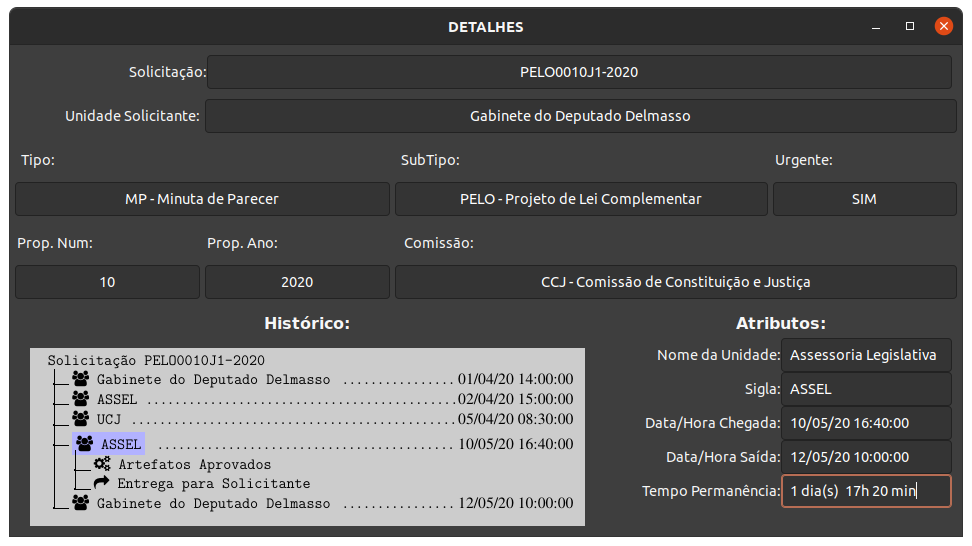
\includegraphics[width=0.99\textwidth]{fig/gerenciaros-detalhar/fig-tela-gerosassel-detalhes-unidade.png}
		\caption{Exemplo de Tela de Detalhe de uma Solicitação onde seleciona-se uma \textbf{Unidade} do \emph{Treeview}.}
		\label{fig:detalhes:unidade}
	\end{figure}

	\begin{figure}[htbp!]
		\centering
		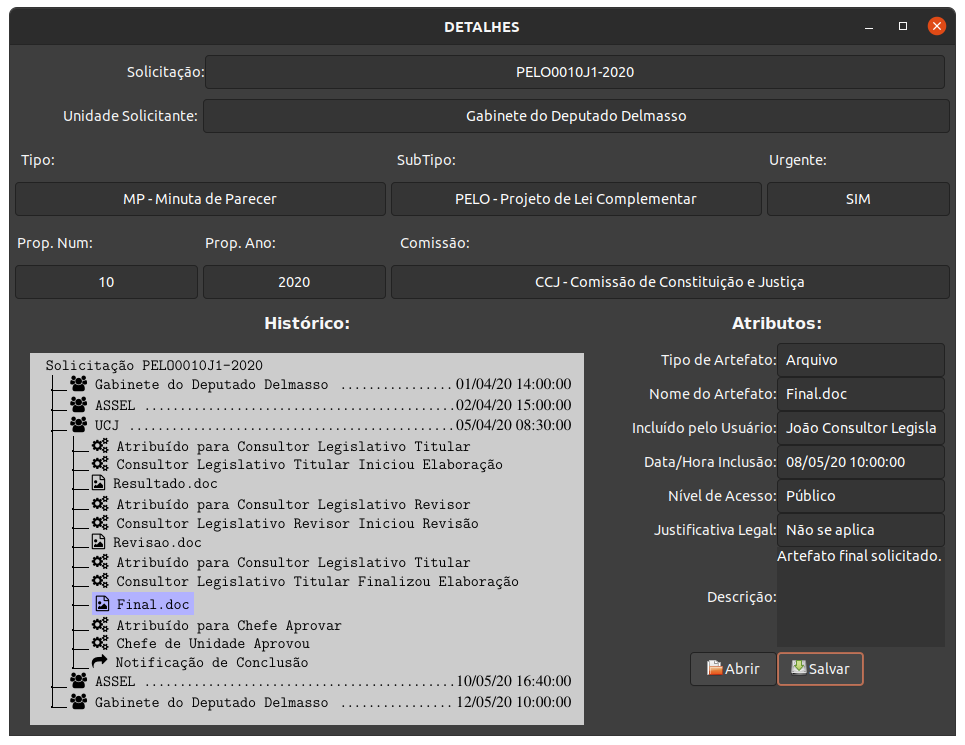
\includegraphics[width=0.99\textwidth]{fig/gerenciaros-detalhar/fig-tela-gerosassel-detalhes-artefato.png}
		\caption{Exemplo de Tela de Detalhe de uma Solicitação onde seleciona-se um \textbf{Artefato} do \emph{Treeview}.}
		\label{fig:detalhes:artefato}
	\end{figure}

	\begin{figure}[htbp!]
	\centering
	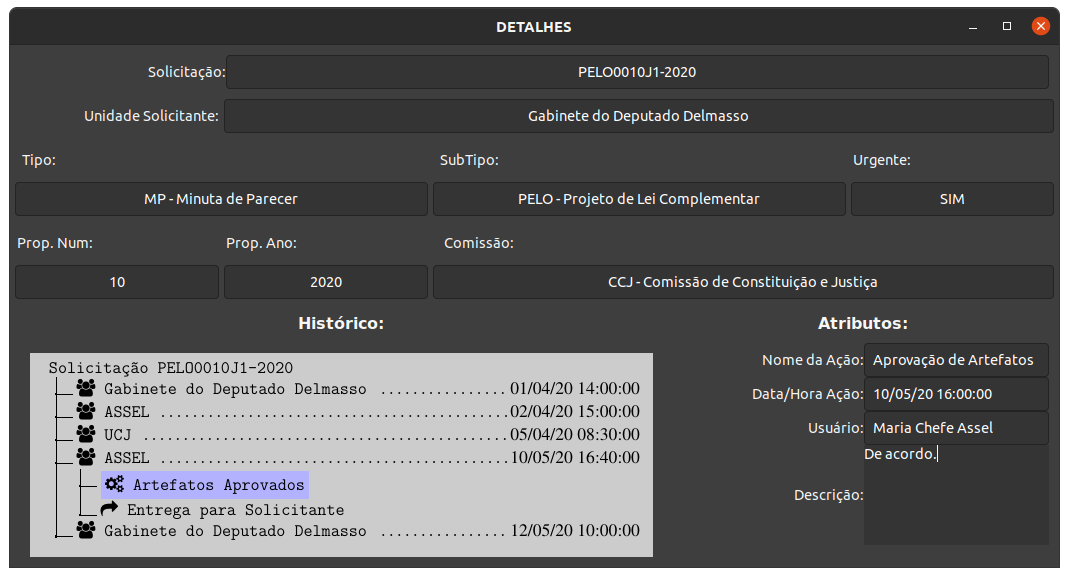
\includegraphics[width=0.99\textwidth]{fig/gerenciaros-detalhar/fig-tela-gerosassel-detalhes-acao.png}
	\caption{Exemplo de Tela de Detalhe de uma Solicitação onde seleciona-se uma \textbf{Ação} do \emph{Treeview}.}
	\label{fig:detalhes:acao}
	\end{figure}

	\begin{figure}[htbp!]
	\centering
	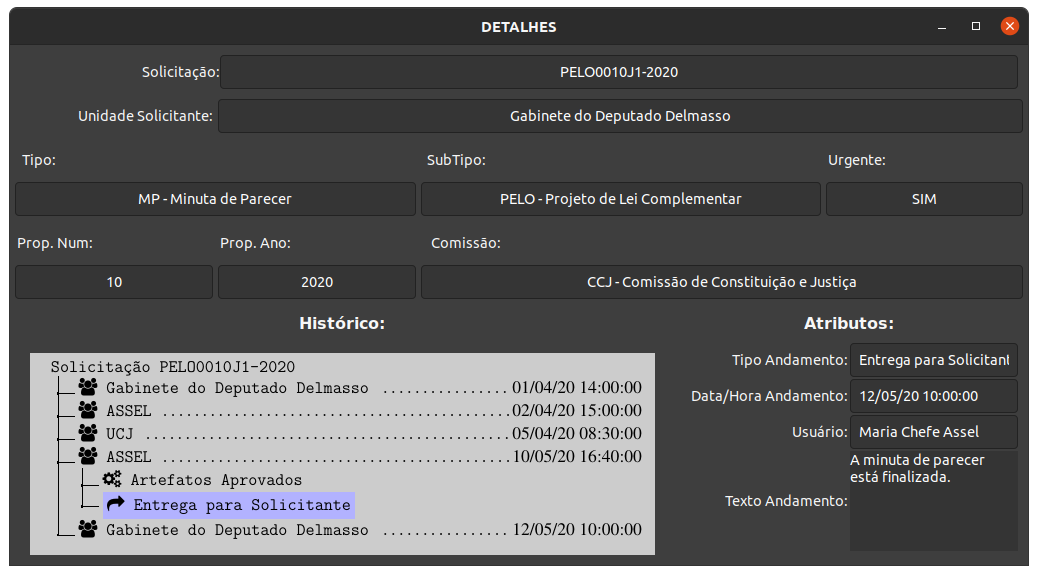
\includegraphics[width=0.99\textwidth]{fig/gerenciaros-detalhar/fig-tela-gerosassel-detalhes-andamento.png}
	\caption{Exemplo de Tela de Detalhe de uma Solicitação onde seleciona-se um \textbf{Andamento} do \emph{Treeview}.}
	\label{fig:detalhes:andamento}
	\end{figure}


	\subsection{Formatos de Arquivos para Janela Detalhar}	
	
	
	Formatos de Arquivos
	
	Coloquei dentro de doc
	
	Preciso criar a nota técnica e pedir para o Gilberto Assinar
	
	 
	





\section{Janela Analisar}

Conforme últimos entendimentos, o conteúdo da janela de Análise vai variar de acordo com os parâmetros da OS escolhida na lista para ser analisada.

%\TODO{Tem que permitir modificar o relator!}


\subsection{Janelas de Análises Possíveis}

Assim, os cenários possíveis são três:

\begin{enumerate}
	\item O \textbf{Andamento} da OS é ``Conclusão'';
	\item O \textbf{Andamento} é qualquer outro exceto ``Conclusão'' e o tipo da OS é Minuta de Parecer;	
	\item O \textbf{Andamento} é qualquer outro exceto ``Conclusão'' e o tipo da OS é qualquer outra exceto Minuta de Parecer.		
\end{enumerate}


\subsubsection{Andamento da OS é ``Conclusão'' e tanto faz o Tipo}

No caso do Andamento ser ``Conclusão'' as funcionalidades necessárias para a Tela de Análise serão:

\begin{nota}[1]{Funcionalidades da Tela de Análise quando: Andamento é ``Conclusão''}
	\begin{itemize}
		\item \textbf{Cabeçalho}: Grupo de Componentes onde informações básicas da OS alvo escolhida para ser analisada são exibidas: Solicitação, Unidade Solicitante, Tipo, Subtipo, Prop,Com, Urgente.
		\item \textbf{Adição de Arquivos}: Poder adicionar novos ``artefatos arquivos'' à solicitação;
		\item \textbf{Adição de Texto}: Poder adicionar novos `'artefatos texto'' à solicitação;
		\item \textbf{Resultado da Análise}: Poder escolher o Resultado da Análise acompanhado de uma mensagem justificando essa escolha.		
	\end{itemize}
\end{nota}


\subsubsection{Andamento da OS não é ``Conclusão'' e Tipo é ``Minuta de Parecer''}

No caso do Andamento \textbf{não} ser ``Conclusão'', mas o Tipo da OS for ``Minuta de Parecer'', então as funcionalidades necessárias para a tela de Análise serão:

\begin{nota}[1]{Funcionalidades da Tela de Análise quando: Andamento não é ``Conclusão'', mas tipo é ``Minuta de Parecer''}
	\begin{itemize}
		\item \textbf{Cabeçalho}: Grupo de Componentes onde informações básicas da OS alvo escolhida para ser analisada são exibidas: Solicitação, Unidade Solicitante, Tipo, Subtipo, Prop,Com, Urgente.
		
		\item \textbf{Proposições Relacionadas}: Grupo de Componentes contendo ``Pesquisa pronta trazendo Solicitações relacionados com a mesma Proposição da MPAR selecionada''. Nesse Grupo de Componentes deve existir:
		
		\begin{itemize}
			\item Tabela com pesquisa ``pronta'' trazendo todos as Solicitações do Sistema cujo Tipo também seja ``Minuta de Parecer'' e cuja Proposição seja a mesma da OS escolhida. 
			\item Opção de escolher dentre as OSs aquelas que serão vinculadas à OS selecionada.
			\item Opção de abrir nova janela ou aba trazendo os Detalhes da OS da tabela de pesquisa selecionada para que essa OS possa ser inspecionada.			
		\end{itemize}			

		\item \textbf{Modificação do Relator}: Grupo de Componentes para criar a opção de modificar o relator da Solicitação de Minuta de Parecer.

		\item \textbf{OSs Vinculadas}: Grupo de Componentes onde podem ser vistos as Solicitações Vinculadas a essa OS Escolhida. Deve-se poder desvincular. Deve-se poder também pesquisar ou escolher e vincular novas OSs à OS alvo.	

		\item \textbf{Modificação de Atributos}: Grupo de Componentes onde deve ser possível modificar os atributos do cabeçalho.

		\item \textbf{Adição de Arquivos}: Poder adicionar novos ``artefatos arquivos'' à solicitação;
		\item \textbf{Adição de Texto}: Poder adicionar novos `'artefatos texto'' à solicitação;

		\item \textbf{Resultado da Análise}: Poder escolher o Resultado da Análise acompanhado de uma mensagem justificando essa escolha.		
	\end{itemize}
\end{nota}



\subsubsection{Andamento da OS não é ``Conclusão'' e  Tipo não é ``Minuta de Parecer''}


No caso do Andamento \textbf{não} ser ``Conclusão''e o Tipo da OS for qualquer outro exceto ``Minuta de Parecer'', então as funcionalidades necessárias para a tela de Análise serão:

\begin{nota}[1]{Funcionalidades da Tela de Análise quando: Andamento não é ``Conclusão'' e tipo não é ``Minuta de Parecer''}
	\begin{itemize}
		\item \textbf{Cabeçalho}: Grupo de Componentes onde informações básicas da OS alvo escolhida para ser analisada são exibidas: Solicitação, Unidade Solicitante, Tipo, Subtipo, Prop,Com, Urgente.

		\item \textbf{OSs Vinculadas}: Grupo de Componentes onde podem ser vistos as Solicitações Vinculadas a essa OS Escolhida. Deve-se poder desvincular. Deve-se poder também pesquisar ou escolher e vincular novas OSs à OS alvo.	
		
		\item \textbf{Modificação de Atributos}: Grupo de Componentes onde deve ser possível poder modificar os atributos do cabeçalho.		
		
		\item \textbf{Adição de Arquivos}: Poder adicionar novos ``artefatos arquivos'' à solicitação;
		
		\item \textbf{Adição de Texto}: Poder adicionar novos `'artefatos texto'' à solicitação;

		\item \textbf{Resultado da Análise}: Poder escolher o Resultado da Análise acompanhado de uma mensagem justificando essa escolha.		
	\end{itemize}
\end{nota}

\subsubsection{Resumo}


\newcommand{\specialcell}[2][c]{%
	\begin{tabular}[#1]{@{}c@{}}#2\end{tabular}}

\begin{table}[!h]
	\begin{center}
		\begin{tabular}{|c|c|c|c|}
			\hline
			\rowcolor{corCOULD!80} \multicolumn{4}{|c|}{\Large Tela de Análise \normalsize} \\ \hline
			\hline
			% CABEÇALHO        
			\rowcolor{lightgray}\textbf{Grupo de Componentes} & \specialcell{\textbf{Andamento}\\\textbf{Conclusão}} & \specialcell{\textbf{Tipo}\\\textbf{é MPAR}} & \specialcell{\textbf{Tipo}\\\textbf{Não é MPAR}} \\ \hline
			% CONTEÚDO
			% Código escrito manualmente
			\rowcolor{corCOULD!20} Cabeçalho & \msmark & \msmark & \msmark \\ \hline
			\rowcolor{cldfC1!40} Proposições Relacionadas & \msnone & \msmark & \msnone \\ \hline
			\rowcolor{cldfC1!40} Modificação de Relator & \msnone & \msmark & \msnone \\ \hline
			\rowcolor{cldfG!40} OSs Vinculadas & \msnone & \msmark & \msmark \\ \hline
			\rowcolor{cldfG!40} Modificação de Atributos & \msnone & \msmark & \msmark \\ \hline
			\rowcolor{corCOULD!20} Adição de Arquivos & \msmark & \msmark & \msmark \\ \hline
			\rowcolor{corCOULD!20} Adição de Texto & \msmark & \msmark & \msmark \\ \hline
			\rowcolor{corCOULD!20} Resultado da Análise & \msmark & \msmark & \msmark \\ \hline
		\end{tabular}    
		\caption{\label{tab:gerosassel:analise:conclusao} Resultados da Análise}
	\end{center}
\end{table}

	Da tabela \ref{tab:gerosassel:analise:conclusao}, conclui-se que:

	\begin{itemize}
		\item Todas as telas de análise terão os grupos de componentes: \textbf{Cabeçalho}, \textbf{Adição de Arquivos}, \textbf{Adição de Textos} e \textbf{Resultado da Análise}.
		\item Somente telas cujo andamento não é conclusão e o tipo for MPAR, terão os grupos \textbf{Proposições Relacionadas} e \textbf{Modificação de Relator}.
		\item Todas as telas de análise cujo andamento não for conclusão deverão apresentar os grupos \textbf{OSs Vinculadas} e \textbf{Modificação de Atributos}. 
	\end{itemize}

\subsection{Tela de Análise com Diversas Abas}

Se utilizarmos a idéia de criar uma janela com diversas Abas, uma aba para cada funcionalidade, e ainda incluir a Tela de Detalhes como uma das abas dessa janela, então, poderíamos pensar em uma só tela com as seguintes abas:


\begin{itemize}
	\item \textbf{Aba Propriedades}: Uma aba com os campos do cabeçalho (Tipo, Subtipo, Urgente, Número da Proposição, Ano da Proposição e Comissão). A funcionalidade de ``Modificação de Atributos'' também seria acessível nesta aba.
	
	
	\item \textbf{Aba Protocolo}: Apresentaria a tela de detalhes conforme descrito nas seções anteriores.
	
	\item \textbf{Aba Proposições}: No caso de MPAR, apresentaria as proposições relacionadas;

	\item \textbf{Aba Relator}: No caso de MPAR, mostraria o Relator vinculado à Solicitação e permitira modificar este Relator; 

	\item \textbf{Aba Relacionamentos}: Mostraria as OSs vinculados a essa Solicitação permitindo pesquisar e vincular outras OSs como também desvincular OSs vinculadas. 

	\item \textbf{Aba para Adição de Textos}: Aba permite adicionar ``Artefato Texto'' à Solicitação.

	\item \textbf{Aba para Adição de Arquivos}: Aba permite adicionar ``Artefatos Arquivos'' à Solicitação.

	\item \textbf{Aba Encaminhamento}: Mostraria o ``Andamento Atual'' e permitiria determinar um ``Andamento Futuro'', ou seja, o ``Resultado da Análise'' e a consequente ``Ação Resultante'';
	
\end{itemize}

A seguir as figuras \ref{fig:analisar:propriedades}, \ref{fig:analisar:protocolo} e \ref{fig:analisar:encaminhamento}  apresentam protótipos de layout de como seriam algumas dessas abas:


	\begin{figure}[h]
		\centering
		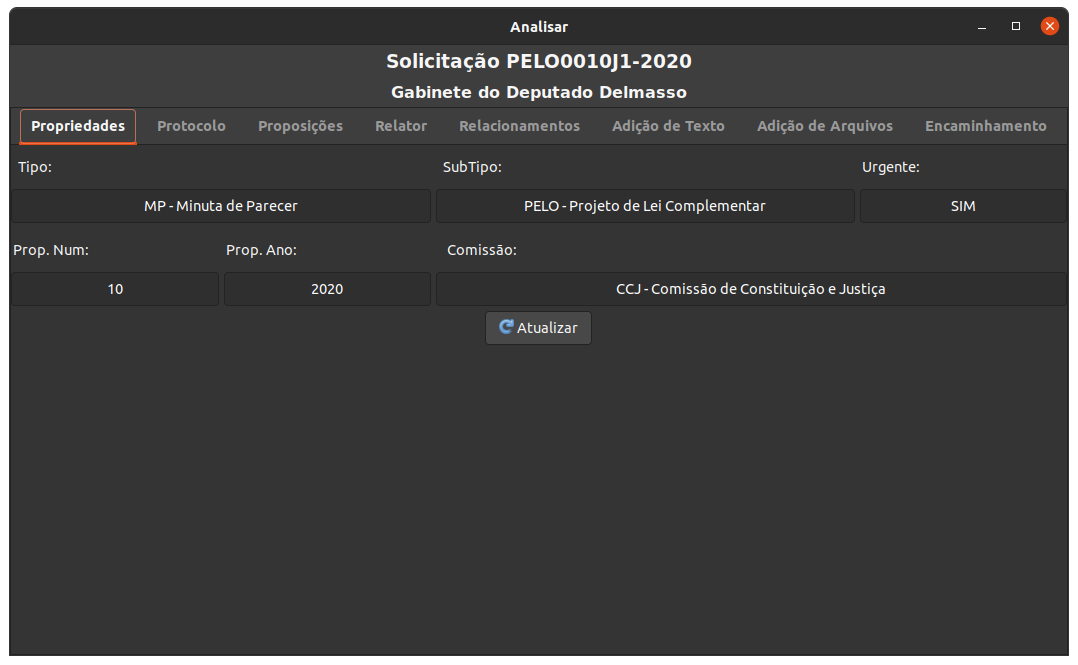
\includegraphics[width=0.9\textwidth]{fig/gerenciaros-analisar/fig-tela-gerosassel-analisar-propriedades.png}
		\caption{\textbf{Aba Propriedades} mostrando os atributos da solicitação e um botão para alterar esses atributos.}
		\label{fig:analisar:propriedades}
	\end{figure}

	\begin{figure}[h]
		\centering
		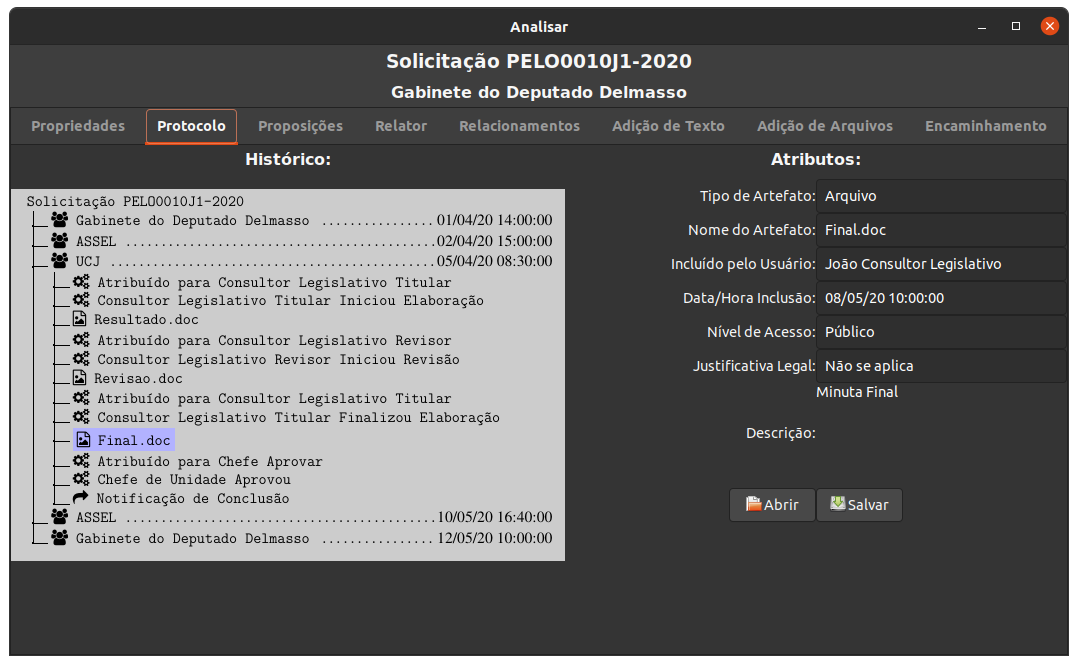
\includegraphics[width=0.9\textwidth]{fig/gerenciaros-analisar/fig-tela-gerosassel-analisar-protocolo.png}
		\caption{\textbf{Aba Protocolo} mostrando os detalhes da solicitação e permitindo abrir ou fazer download de arquivos.}
		\label{fig:analisar:protocolo}
	\end{figure}

	\begin{figure}[htbp!]
		\centering
		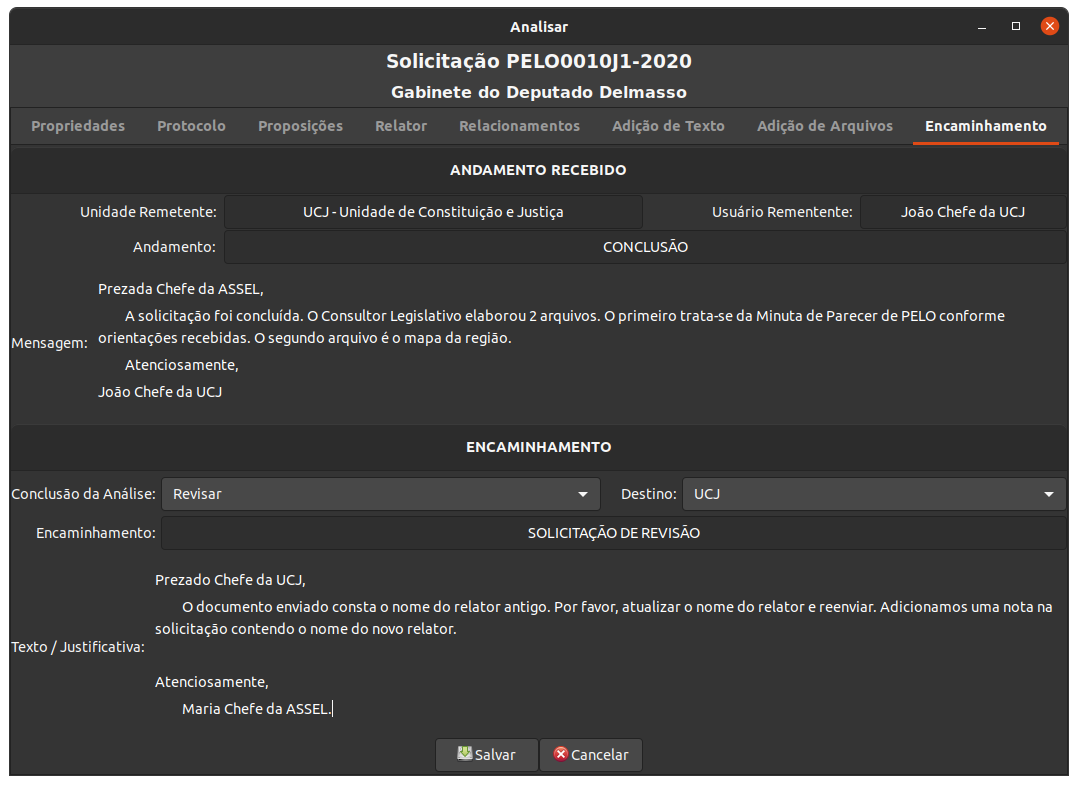
\includegraphics[width=0.9\textwidth]{fig/gerenciaros-analisar/fig-tela-gerosassel-analisar-encaminhamento.png}
		\caption{\textbf{Aba Encaminhamento} apresentando o andamento atual e permitindo-se escolher o andamento futuro (encaminhamento) da Solicitação.}
		\label{fig:analisar:encaminhamento}
	\end{figure}


\subsection{Resultados Possíveis para as Análises}


\subsubsection{Andamento da OS é ``Conclusão''}

Nesse caso, as possibilidades de ``Resultados para a Análise'' e consequente ``Ação Resultante'' deverão ser:

\begin{table}[!h]
	\begin{center}
		\begin{tabular}{|c|c|c|}
			\hline
			\rowcolor{corCOULD!80} \multicolumn{3}{|c|}{\Large Andamento da OS é ``Conclusão'' \normalsize} \\ \hline
			\hline
			\rowcolor{corCOULD!40} \multicolumn{3}{|c|}{\Large Opções de Análise, Destino e Ações Resultantes  \normalsize} \\ \hline \hline
			% CABEÇALHO        
			\rowcolor{lightgray}\textbf{Opção de Análise} & \textbf{Destino Resultante} & \textbf{Ação Resultante} \\ \hline
			% CONTEÚDO
			% Código escrito manualmente
			\rowcolor{cldfC1!40} \cellcolor{corCOULD!10} Concluir & Solicitante & Serviço Concluído \\ \hline
			\rowcolor{cldfC1!40} \cellcolor{corCOULD!10} Revisar & Remetente & Solicitação de Revisão \\ \hline
		\end{tabular}    
		\caption{\label{tab:gerosassel:analise1} Resultados da Análise}
	\end{center}
\end{table}

\subsubsection{Andamento da OS não é ``Conclusão''}


Finalmente, quando o andamento da OS não é ``Conclusão'' \textbf{qualquer que seja o Tipo}, as possibilidades de ``Análise'' e consequente ``Ação Resultante'' deverão ser:

\begin{table}[!h]
	\begin{center}
		\begin{tabular}{|c|c|c|}
			\hline
			\rowcolor{corCOULD!80} \multicolumn{3}{|c|}{\Large Andamento \textbf{não} é ``Conclusão'' e Tipo é ``Minuta de Parecer'' \normalsize} \\ \hline
			\hline
			\rowcolor{corCOULD!40} \multicolumn{3}{|c|}{\Large Opções de Análise, Destino Escolhido e Ações Resultantes  \normalsize} \\ \hline \hline
			% CABEÇALHO        
			\rowcolor{lightgray}\textbf{Opção de Análise} & \textbf{Destino Escolhido} & \textbf{Ação Resultante} \\ \hline
			% CONTEÚDO
			% Código escrito manualmente
			\rowcolor{cldfC1!40} \cellcolor{corCOULD!10} Cancelar & Tanto Faz & Cancelar \\ \hline
			\rowcolor{cldfC1!40} \cellcolor{corCOULD!10} Solicitar Pendência & Tanto Faz & Solicitação de Pendência \\ \hline
			\rowcolor{cldfC1!40} \cellcolor{corCOULD!10} Distribuir & Não Especificado & Indefinido \\ \hline
			\rowcolor{cldfC1!40} \cellcolor{corCOULD!10} Distribuir & Especificado & Distribuir \\ \hline
		\end{tabular}    
		\caption{\label{tab:gerosassel:analise2} Resultados da Análise}
	\end{center}
\end{table}


\textbf{Observações:}
\begin{itemize}
	\item O ``Destino Escolhido'' é o Destino que pode ser escolhido na Tela Principal, geralmente pelo Perfil de Supervisor. Dessa forma, o valor do campo Destino deve vir de lá. Porém, ele pode ser alterado aqui.
\end{itemize}

As opções possíveis de ``Destino'' devem ser:

\begin{nota}[1]{Opções de Destinos}
	\begin{itemize}
		\item Não Especificado - Quando o destino não foi especificado ainda pois aguarda-se que outro usuário faça essa escolha.
		\item UCJ - Unidade de Constituição e Justiça;
		\item URP - Unidade de Redação Parlamentar e Consolidação dos Textos Legislativos;
		\item UEF - Unidade de Economia e Finanças;
		\item USE - Unidade de Saúde, Educação, Cultura e Desenvolvimento Científico e Tecnológico; 
		\item UDA - Unidade de Desenvolvimento Urbano e Rural e Meio Ambiente;	
	\end{itemize}
\end{nota}


\section{Figuras Auxiliares}


\begin{figure}[htbp!]
	\begin{adjustbox}{minipage=\linewidth,bgcolor=gray!40,varwidth=\linewidth-10pt}    	
		
		\vphantom{}
		
		\dirtree{%
			.1 Solicitação PELO0010J1-2020.
			.2 \msUnd Gabinete do Deputado Delmasso \DTcomment{01/04/20 14:00:00}. 
			.2 \msUnd ASSEL \DTcomment{02/04/20 15:00:00}.
			.2 \msUnd UCJ \DTcomment{05/04/20 08:30:00}.
			.2 \colorbox{blue!30}{\msUnd ASSEL} \DTcomment{10/05/20 16:40:00}.
			.3 \msAct Artefatos Aprovados.
			.3 \msAnd Entrega para Solicitante.
			.2 \msUnd Gabinete do Deputado Delmasso \DTcomment{12/05/20 10:00:00}.
		}
		
		\vphantom{}
		
	\end{adjustbox}
	\caption{Exemplo na qual a Unidade ``ASSEL'' está selecionada.}
	\label{tree:ex5}
\end{figure}	




\begin{figure}[htbp!]
	\begin{adjustbox}{minipage=\linewidth,bgcolor=gray!40,varwidth=\linewidth-10pt}    	
		
		\vphantom{}
		
		\dirtree{%
			.1 Solicitação PELO0010J1-2020.
			.2 \msUnd Gabinete do Deputado Delmasso \DTcomment{01/04/20 14:00:00}. 
			.2 \msUnd ASSEL \DTcomment{02/04/20 15:00:00}.
			.2 \msUnd UCJ \DTcomment{05/04/20 08:30:00}.
			.3 \msAct Atribuído para Consultor Legislativo Titular.
			.3 \msAct Consultor Legislativo Titular Iniciou Elaboração.
			.3 \msArt Resultado.doc.
			.3 \msAct Atribuído para Consultor Legislativo Revisor.
			.3 \msAct Consultor Legislativo Revisor Iniciou Revisão.
			.3 \msArt Revisao.doc.
			.3 \msAct Atribuído para Consultor Legislativo Titular.
			.3 \msAct Consultor Legislativo Titular Finalizou Elaboração.
			.3 \colorbox{blue!30}{\msArt Final.doc}.
			.3 \msAct Atribuído para Chefe Aprovar.
			.3 \msAct Chefe de Unidade Aprovou. 
			.3 \msAnd Notificação de Conclusão. 
			.2 \msUnd ASSEL \DTcomment{10/05/20 16:40:00}.
			.2 \msUnd Gabinete do Deputado Delmasso \DTcomment{12/05/20 10:00:00}.
		}
		
		\vphantom{}
		
	\end{adjustbox}
	\caption{Exemplo na qual o Artefato ``Final.doc'' está selecionado.}
	\label{tree:ex6}
\end{figure}	



\begin{figure}[htbp!]
	\begin{adjustbox}{minipage=\linewidth,bgcolor=gray!40,varwidth=\linewidth-10pt}    	
		
		\vphantom{}
		
		\dirtree{%
			.1 Solicitação PELO0010J1-2020.
			.2 \msUnd Gabinete do Deputado Delmasso \DTcomment{01/04/20 14:00:00}. 
			.2 \msUnd ASSEL \DTcomment{02/04/20 15:00:00}.
			.2 \msUnd UCJ \DTcomment{05/04/20 08:30:00}.
			.2 \msUnd ASSEL \DTcomment{10/05/20 16:40:00}.
			.3 \colorbox{blue!30}{\msAct Artefatos Aprovados}.
			.3 \msAnd Entrega para Solicitante.
			.2 \msUnd Gabinete do Deputado Delmasso \DTcomment{12/05/20 10:00:00}.
		}
		
		\vphantom{}
		
	\end{adjustbox}
	\caption{Exemplo na qual a Ação ``Artefatos Aprovados'' está selecionado.}
	\label{tree:ex7}
\end{figure}	



\begin{figure}[htbp!]
	\begin{adjustbox}{minipage=\linewidth,bgcolor=gray!40,varwidth=\linewidth-10pt}    	
		
		\vphantom{}
		
		\dirtree{%
			.1 Solicitação PELO0010J1-2020.
			.2 \msUnd Gabinete do Deputado Delmasso \DTcomment{01/04/20 14:00:00}. 
			.2 \msUnd ASSEL \DTcomment{02/04/20 15:00:00}.
			.2 \msUnd UCJ \DTcomment{05/04/20 08:30:00}.
			.2 \msUnd ASSEL \DTcomment{10/05/20 16:40:00}.
			.3 \msAct Artefatos Aprovados.
			.3 \colorbox{blue!30}{\msAnd Entrega para Solicitante}.
			.2 \msUnd Gabinete do Deputado Delmasso \DTcomment{12/05/20 10:00:00}.
		}
		
		\vphantom{}
		
	\end{adjustbox}
	\caption{Exemplo na qual o Andamento ``'Entrega para Solicitante' está selecionado.}
	\label{tree:ex8}
\end{figure}	





























	


